\documentclass[10pt]{gulartcl}
\usepackage{../exstyle}

\title{Esercizio settimanale n. 3}
\author{Guglielmo Bordin}
\date{\today}

\begin{document}
\maketitle
    
\noindent
Quattro particelle cariche di massa $m$ e carica $q$, tre positive e una
negativa, sono poste ai vertici di un quadrato di lato $\ell$ come mostrato
in figura. La particella in alto a destra viene poi rilasciata, lasciando
le altre vincolate al loro posto. 
\begin{enumerate}
    \item Dove si dirigerà? Indicare la direzione come angolo rispetto
        all’orizzontale.
    \item Che velocità avrà quando si troverà a grandissima distanza dalle
        altre cariche?
\end{enumerate}

\bigbreak
\begin{center}
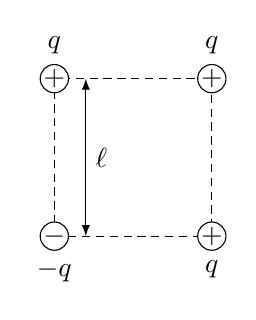
\begin{tikzpicture}
    \draw[densely dashed] (0, 0) -- (2, 0) -- (2, 2) -- (0, 2) -- cycle;
    \node[inner sep=0pt, circle, draw, fill=white, label={below:{$-q$}}]
        at (0, 0) {$-$};
    \node[inner sep=0pt, circle, draw, fill=white, label={below:{$q$}}]
        at (2, 0) {$+$};
    \node[inner sep=0pt, circle, draw, fill=white, label={above:{$q$}}]
        at (0, 2) {$+$};
    \node[inner sep=0pt, circle, draw, fill=white, label={above:{$q$}}]
        at (2, 2) {$+$};
    \draw[latex-latex] (0.4, 0) -- ++(0, 2) node[midway, anchor=west]
        {$\ell$};
\end{tikzpicture} 
\end{center}
\end{document}
